\chapter{YUL Optimizer Deep Dive}
\section{Optimization flow}
\paragraph*{}
As seen in the solidity compilation flow \ref{fig:solc-compilation-flow}, solidity optimizes its code via an \textbf{optimizer suite} which runs against the YUL IR. This consists of currently 32 documented steps \cite{solidity-yul-optimizer}, followed by a series of bytecode (opcode) optimizations which we will not focus on in this chapter. Some of the optimization steps are required to be run first, as they impose a specific structure to be further used and also make it safe to run arbitrary sequences of optimization steps \cite{solidity-yul-optimizer}, and are run in the following order:
\begin{enumerate}
    \item \textbf{Disambiguator}: returns a copy of the YUL AST where each variable has a unique identifier. Therefore, an AST walker can maintain a global state with regards to all of the identifiers in the code, even if we have variables with the same name in different parts of the program. This property is maintained by any subsequent step and there are no identical identifier names introduced while optimizing.
    \item \textbf{FunctionHoister}: moves all function definitions to the topmost block to enable isolated optimization of function definitions.
    \item \textbf{FunctionGrouper}: reorders code, such that the YUL code is of the form ${I \ F\ldots}$, where $I$ are instructions of the (possibly empty) entry block in the CFG and $F$ contain \textbf{un-nested} function definitions.
    \item \textbf{BlockFlattener} flattens nested blocks of code of form $\{\{ B \}\}$ to $\{ B \}$ if possible, i.e. if no interrupting control flows appear between the code blocks.
\end{enumerate}

% All components of the Yul-based optimizer module are explained below. The following transformation steps are the main components:

% SSA Transform

% Common Subexpression Eliminator

% Expression Simplifier

% Redundant Assign Eliminator

% Full Inliner


\paragraph*{}
Optimization makes a big difference. In code sample \ref{code:variable-declaration} we compute gas cost to re-declare a variable inside a for loop. When not optimized, the execution gast cost estimates for running \lstinline[language=Solidity]{declareVariableOutsideLoop} is $415250$ gas and \\ \lstinline[language=Solidity]{declareVariableInsideLoop} is $420223$ gas. This is expected, since the latter re-declares the same variable in every loop iteration.

\paragraph*{}
When optimized, however, gas usage is almost four times better, with \\ \lstinline[columns=fixed, language=Solidity]{declareVariableOutsideLoop} estimated to $119194$ gas and \lstinline[columns=fixed, language=Solidity]{declareVariableInsideLoop} to $119211$. An important note here is that the gas difference comes from the \textbf{function dispatch}, as described by Hari Mulackal \cite{hari-gas-dispatch}, i.e. the order of the functions in a contract introduce a small overhead. Specifically for this case, the optimization comes from the LoopInvariantCodeMotion step, which moves declarations (not assignments) outside the for loop.


\label{code:variable-declaration}
\begin{lstlisting}[language=Solidity, caption=Code example of bad variable declaration inside a for loop]
    // SPDX-License-Identifier: MIT
    pragma solidity ^0.8.14;

    contract VariableLoop {
        function declareVariableInsideLoop() public pure {
            for (uint i = 1; i <= 1000; i++) {
                uint x = i * i;
            }
        }

        function declareVariableOutsideLoop() public pure {
            uint x;
            for (uint i = 1; i <= 1000; i++) {
                x = i * i;
            }
        }
    }
\end{lstlisting}

\paragraph*{}
\textbf{Order matters} when running the optimization steps. In version 0.8.14, the default order \footnote{Optimization order is given by the step abbreviations, where each letter corresponds to an optimization phase. The mapping is described in the \href{https://docs.soliditylang.org/en/v0.8.14/yul.html}{Optimization Step Sequence section in the documentation}.} of the suite is

\begin{lstlisting}
    dhfoDgvulfnTUtnIf[xa[r]EscLMcCTUtTOntnfDIulLculVcul [j]Tpeulxa[rul]xa[r]cLgvifCTUca[r]LSsTFOtfDnca[r]Iulc]jmul[jul] VcTOcul jmul
\end{lstlisting}

In the above order, the optimizers between brackets \cite[will be applied multiple times in a loop until the Yul code remains unchanged or until the maximum number of rounds (currently 12)]{solidity-yul-optimizer}. We can immediately see that some of the optimizers are run more than once, the reasoning being that each optimizer may change the YUL IR, therefore giving new optimization opportunities to other optimizer. This is the case for UnusedAssignEliminator (r abbreviation) and UnusedPruner (u abbreviation). For example, let's optimize the following code in 2 rounds, first applying UnusedPruner and then UnusedAssignEliminator, then applying UnusedAssignEliminator and then UnusedPruner \footnote{The corresponding commands are \lstinline[columns=fixed]{solc --optimize --ir-optimized --via-ir --yul-optimizations 'ur' termination.sol} and \lstinline[columns=fixed]{solc --optimize --ir-optimized --via-ir --yul-optimizations 'ru' termination.sol}}:


\label{code:solidity-redundant-assignment}
\begin{lstlisting}[language=Solidity, caption=Example of a smart contract with a redundant assignment and variable declaration]
    // SPDX-License-Identifier: MIT
    pragma solidity ^0.8.14;

    contract Termination {
        uint persistent_var;
        event FunctionCalled(string f);

        function assignBeforeTermination() public {
            emit FunctionCalled("assignBeforeTermination");
            uint balance;
            balance = 7919;
            return;
        }
    }
\end{lstlisting}


\begin{figure}
    \centering
    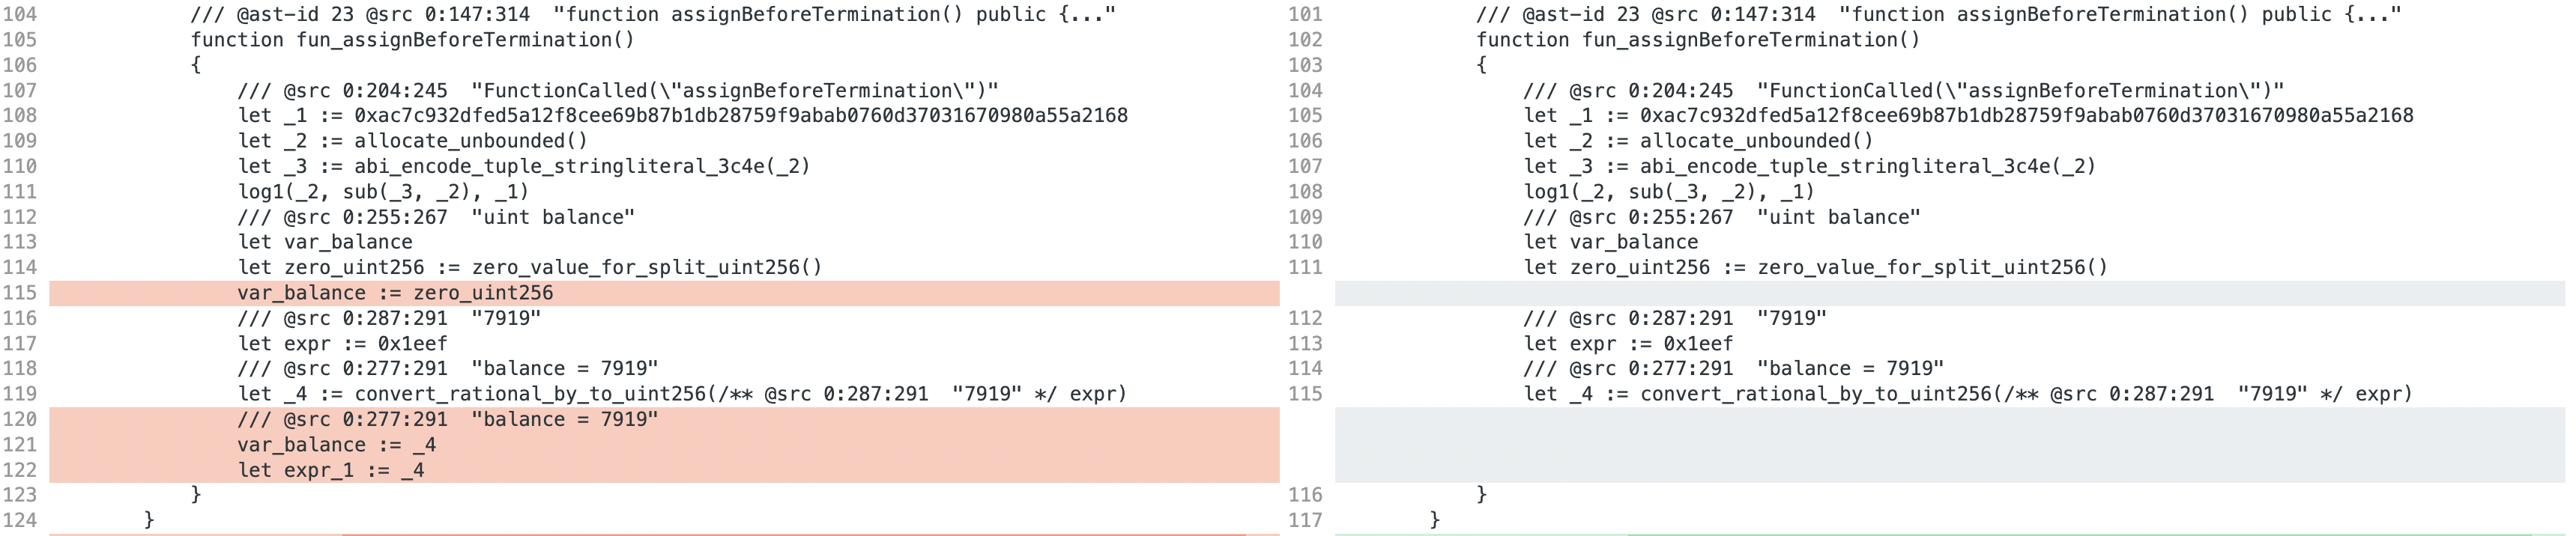
\includegraphics[width=\textwidth]{images/optimization_order_ur.png}
    \caption{Unoptimized vs. optimized YUL IR for Solidity code \ref{code:solidity-redundant-assignment}, order of optimizers: UnusedPruner then UnusedAssignEliminator}
    \label{fig:optimization-order-ur}
\end{figure}

\begin{figure}
    \centering
    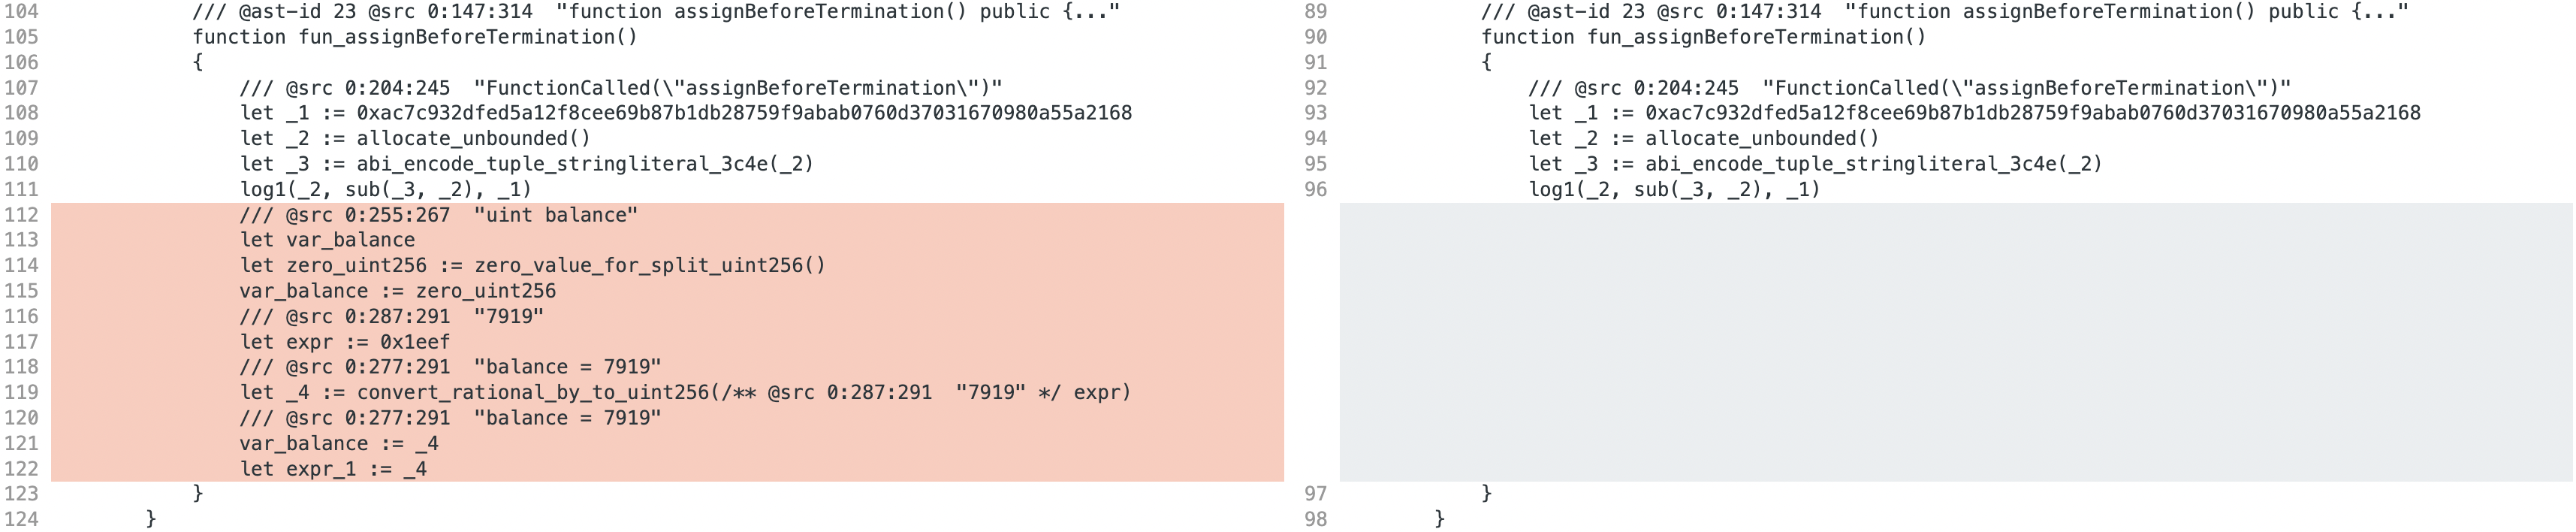
\includegraphics[width=\textwidth]{images/optimization_order_ru.png}
    \caption{Unoptimized vs. optimized YUL IR for Solidity code \ref{code:solidity-redundant-assignment}, order of optimizers: UnusedAssignEliminator then UnusedPruner}
    \label{fig:optimization-order-ru}
\end{figure}


\paragraph*{}
In the above figures \ref{fig:optimization-order-ru} \ref{fig:optimization-order-ur}, we have the same unoptimized YUL IR in the left-hand side, with the optimized YUL code on the right. Upon applying UnusedPruner, this step will look to remove any variable declarations that are not used. When applied first, it correctly identifies \lstinline[columns=fixed]{let expr_1 := _4} as a redundant variable declaration and it removes it. Afterwards, UnusedAssignEliminator runs and it finds \lstinline[columns=fixed]{var_balance := zero_uint256} and \lstinline[columns=fixed]{var_balance := _4} as redundant assignments and removes those as well. However, we can still notice some left-over assignments and variable declarations.

\paragraph*{}
If, however, UnusedAssignEliminator is run first, it removes the same assignments (\lstinline[columns=fixed]{var_balance := zero_uint256} and \lstinline[columns=fixed]{var_balance := _4}), but then gives more room for UnusedPruner to act. Therefore, all of the variable declarations get removed, since their values are not used and they are redundant.

\paragraph*{}
While this is a proof-of-concept example, optimizer steps frequently generate intermediary data objects (such as the SSATransform) to make local optimizations safe and possible (remember that corectness comes before optimization). Hence why these two optimizers are simple, yet effective.

\section{UnusedPruner. UnusedAssignEliminator.}
\paragraph*{}
A very effective way of reducing gas usage is by removing any kind of redundant variable assignments or variable declarations, since it implies executing less instructions. This can be applied as both a local optimization and as a global optimization. In case we locally prune variable declarations, we must ensure that other control flows do not have references to the the left-hand side of the assignment. For example, considering \ref*{code:assignment-sample}, we can see that the assignment at line 3 can be removed, since \lstinline[columns=fixed]{a} is immediately re-assigned. However, even though \lstinline[columns=fixed]{a} gets re-assigned at line 10, we cannot remove assignment at line 4, because there is another control flow that uses the latter assignment, in the \lstinline[columns=fixed]{if} statement. 

\label{code:assignment-sample}
\begin{lstlisting}[caption=YUL IR code sample for variable assignments. Both variables a and b are used in a different control flow.]
{
    let a
    a := 1
    a := 2
    b := 2
    if calldataload(0)
    {
        b := mload(a)
    }
    a := b
}
\end{lstlisting}

\subsection{Variable states in UnusedAssignEliminator}
\paragraph*{}
UnusedAssignEliminator acts in two phases: one to collect information and one to prune redundant assignments. While doing data flow analysis, it assigns different states to the identifiers \footnote{This optimizer only treats assignment where the left-hand side is a single identifier (variable)}: \textbf{undecided, used and unused}. It does so by acting as an YUL AST walker and visiting each VariableAssignment node. On the second pass, any assignment expression that is in the ``undecided'' state will be marked as ``unused'' and will be pruned from the AST, therefore from the final YUL IR code.

\paragraph*{}
An assignment \lstinline[columns=fixed]{a := b} will be marked as ``used'' only if there exists another expression $E$ within the same basic block $B$ or within a basic block $B'$ such that we have a path in the CFG from $B$ to $B'$, where $E$ contains \lstinline[columns=fixed]{a} on the right-hand side. Similarly, if such an expression $E$ does not exist, then the assignment can be marked as ``unused''.


\section{Handling termination flows}
\paragraph*{}
While getting acquainted with the compiler, several experiments have pointed out that the compiler does not treat all of the edge cases with regards to redundant assignments, especially when \textbf{termination flows} appear within basic blocks. YUL IR uses the EVM dialect where termination flows are given by the \lstinline[columns=fixed]{return}, \lstinline[columns=fixed]{revert}, \lstinline[columns=fixed]{selfdestruct} and \lstinline[columns=fixed]{invalid} instructions \footnote{It suffices to focus on the YUL IR instructions, since the optimization flow does not work with Solidity code directly.}. To understand the examples, we must note the different control flows that are present in the CFG for the YUL AST: FlowOut, Break, Continue, Terminate and Leave.

\begin{figure}
    \centering
    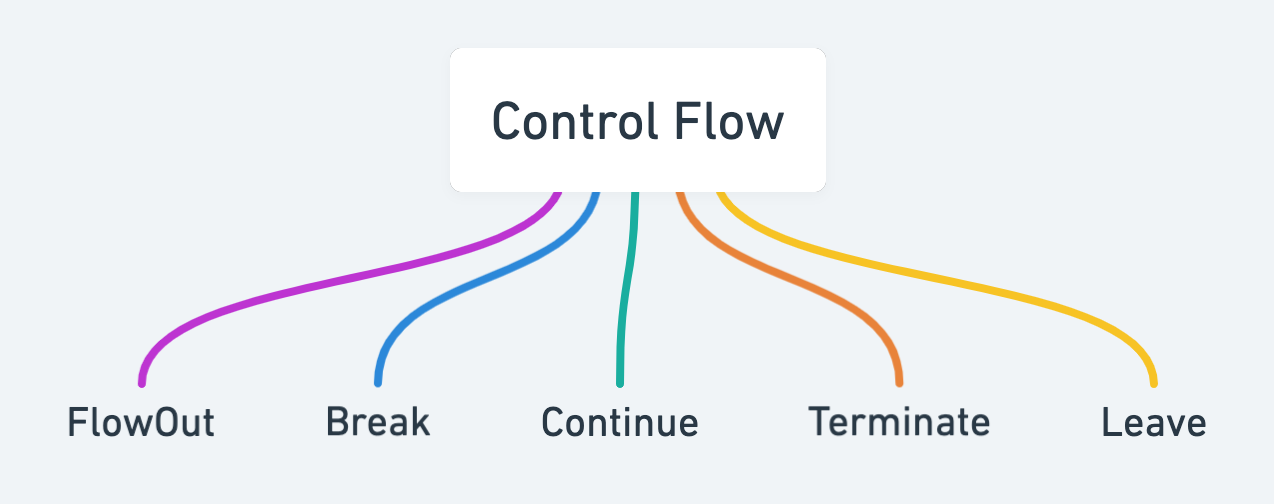
\includegraphics[width=10cm]{images/cfg_control_flow_types.png}
    \caption{Control flow types in YUL IR}
    \label{fig:cfg-control-flow-types}
\end{figure}

\paragraph*{}
All of the above except FlowOut are applied to simple, one-line statements. FlowOut is the most complex one and it embeds the normal execution of the program, as well as the terminal execution of a program. It is applied ``by default`` to \lstinline[columns=fixed]{for} loops \footnote{In YUL IR, \lstinline[columns=fixed]{while} loops get converted to \lstinline[columns=fixed]{for} loops}, \lstinline[columns=fixed]{if} statements, \lstinline[columns=fixed]{switch} statements and functions that can revert, stop or exit normally upon calling them.

\paragraph*{}
A successful attempt to ``fool'' the compiler was done by introducing a Terminate control flow after a redundant assign eliminator. The code sample is as follows:

\label{code:unused-assign-eliminator-handle-termination-flow}
\begin{lstlisting}[caption=YUL IR code sample for variable assignments. Both variables a and b are used in a different control flow.]
    // SPDX-License-Identifier: MIT
    pragma solidity ^0.8.14;
    
    contract Termination {
        uint persistent_var;
        event FunctionCalled(string f);
        event BalanceIsEmpty();
    
        function assignBeforeTermination(uint x) public {
            emit FunctionCalled("assignBeforeTermination");
            uint balance;
            
            if (f1(x) == true) {
                balance = 10007;
                return;
            }
    
            if (balance == 0) {
                emit BalanceIsEmpty();
            }
            return;
        }
    
        function f1(uint x) public pure returns (bool) {
            return x > 10;
        }
    }    
\end{lstlisting}

The introduced termination flow is at line 15, right after the assignment to variable \lstinline[columns=fixed]{balance}, which is then referenced inside the second \lstinline[columns=fixed]{if} condition. The usage of \lstinline[columns=fixed]{f1} functions is necessary to make it impossible for the compiler to compute the \lstinline[columns=fixed]{if} condition's value at compile time, i.e. introduce a \textbf{non-deterministic} flow. The compiler seens \lstinline[columns=fixed]{balance} as referenced in a different control flow, therefore it will not remove assignment at line 14. We can easily see, however, that if the condition \lstinline[columns=fixed]{f1(x) == true} does not stand, then the second if will always evaluate to true, hence why the StructuralSimplifier optimizer could be used to simplify things further and entirely remove the second if condition, since it will always evaluate be true if the termination flow is not executed.


\begin{figure}
    \centering
    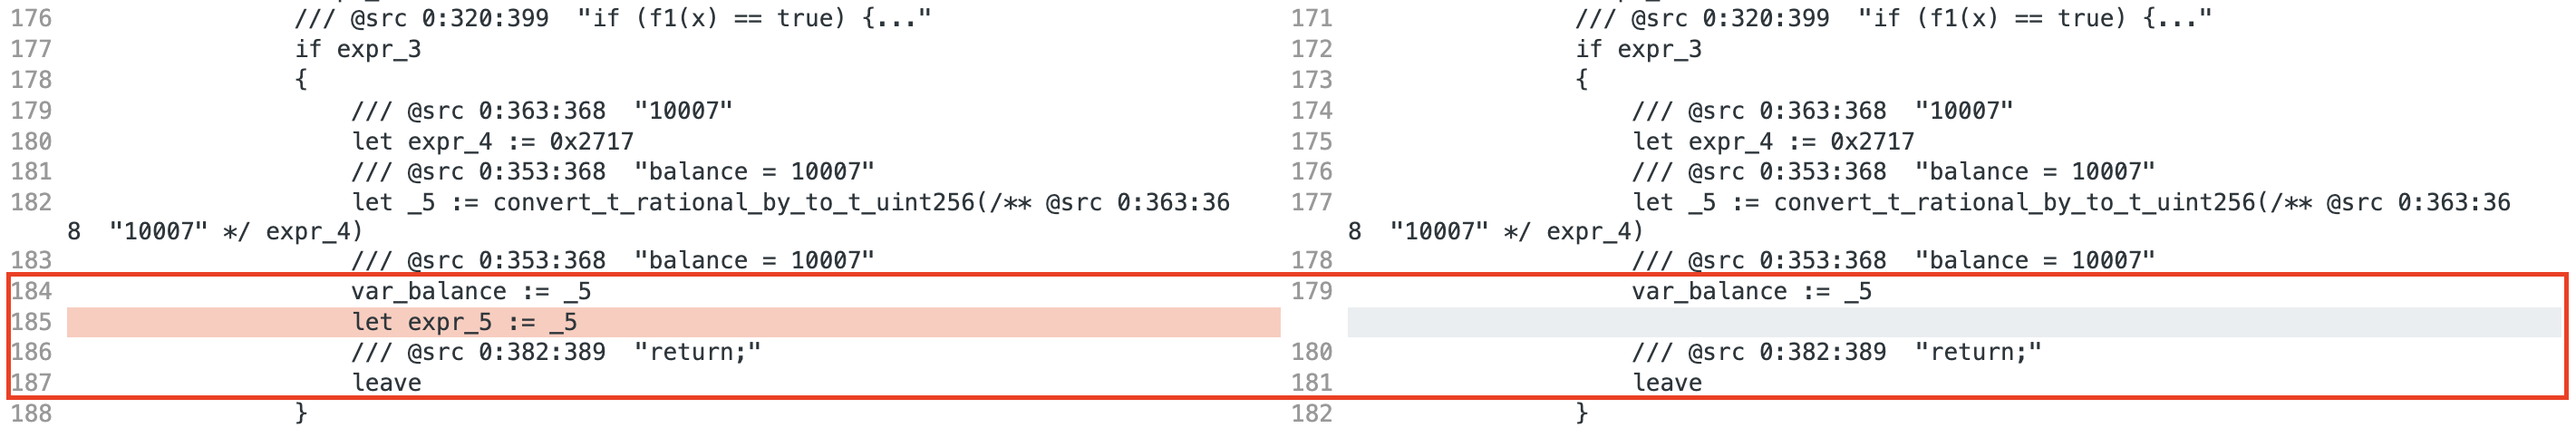
\includegraphics[width=\textwidth]{images/unused_assign_eliminator_termination2.png}
    \caption{Optimized YUL IR using UnusedAssignEliminator then UnusedPruner. UnusedAssignEliminator does not handle termination flows while pruning}
    \label{fig:unused-assign-eliminator-termination2}
\end{figure}

\paragraph*{}
To handle this edge case, we can simplify the problem of determining wether a basic block contains a termination flow or not. Figure \ref*{fig:basic-block-termination-ast-example} shows how a \lstinline[columns=fixed]{leave} statement could be following by valid YUL IR statements (i.e. dead Solidity code after a \lstinline[columns=fixed]{return} instruction). We use the DeadCodeEliminator step for this case to ensure that there are no instructions following an instruction that terminates the execution.

\begin{figure}
    \centering
    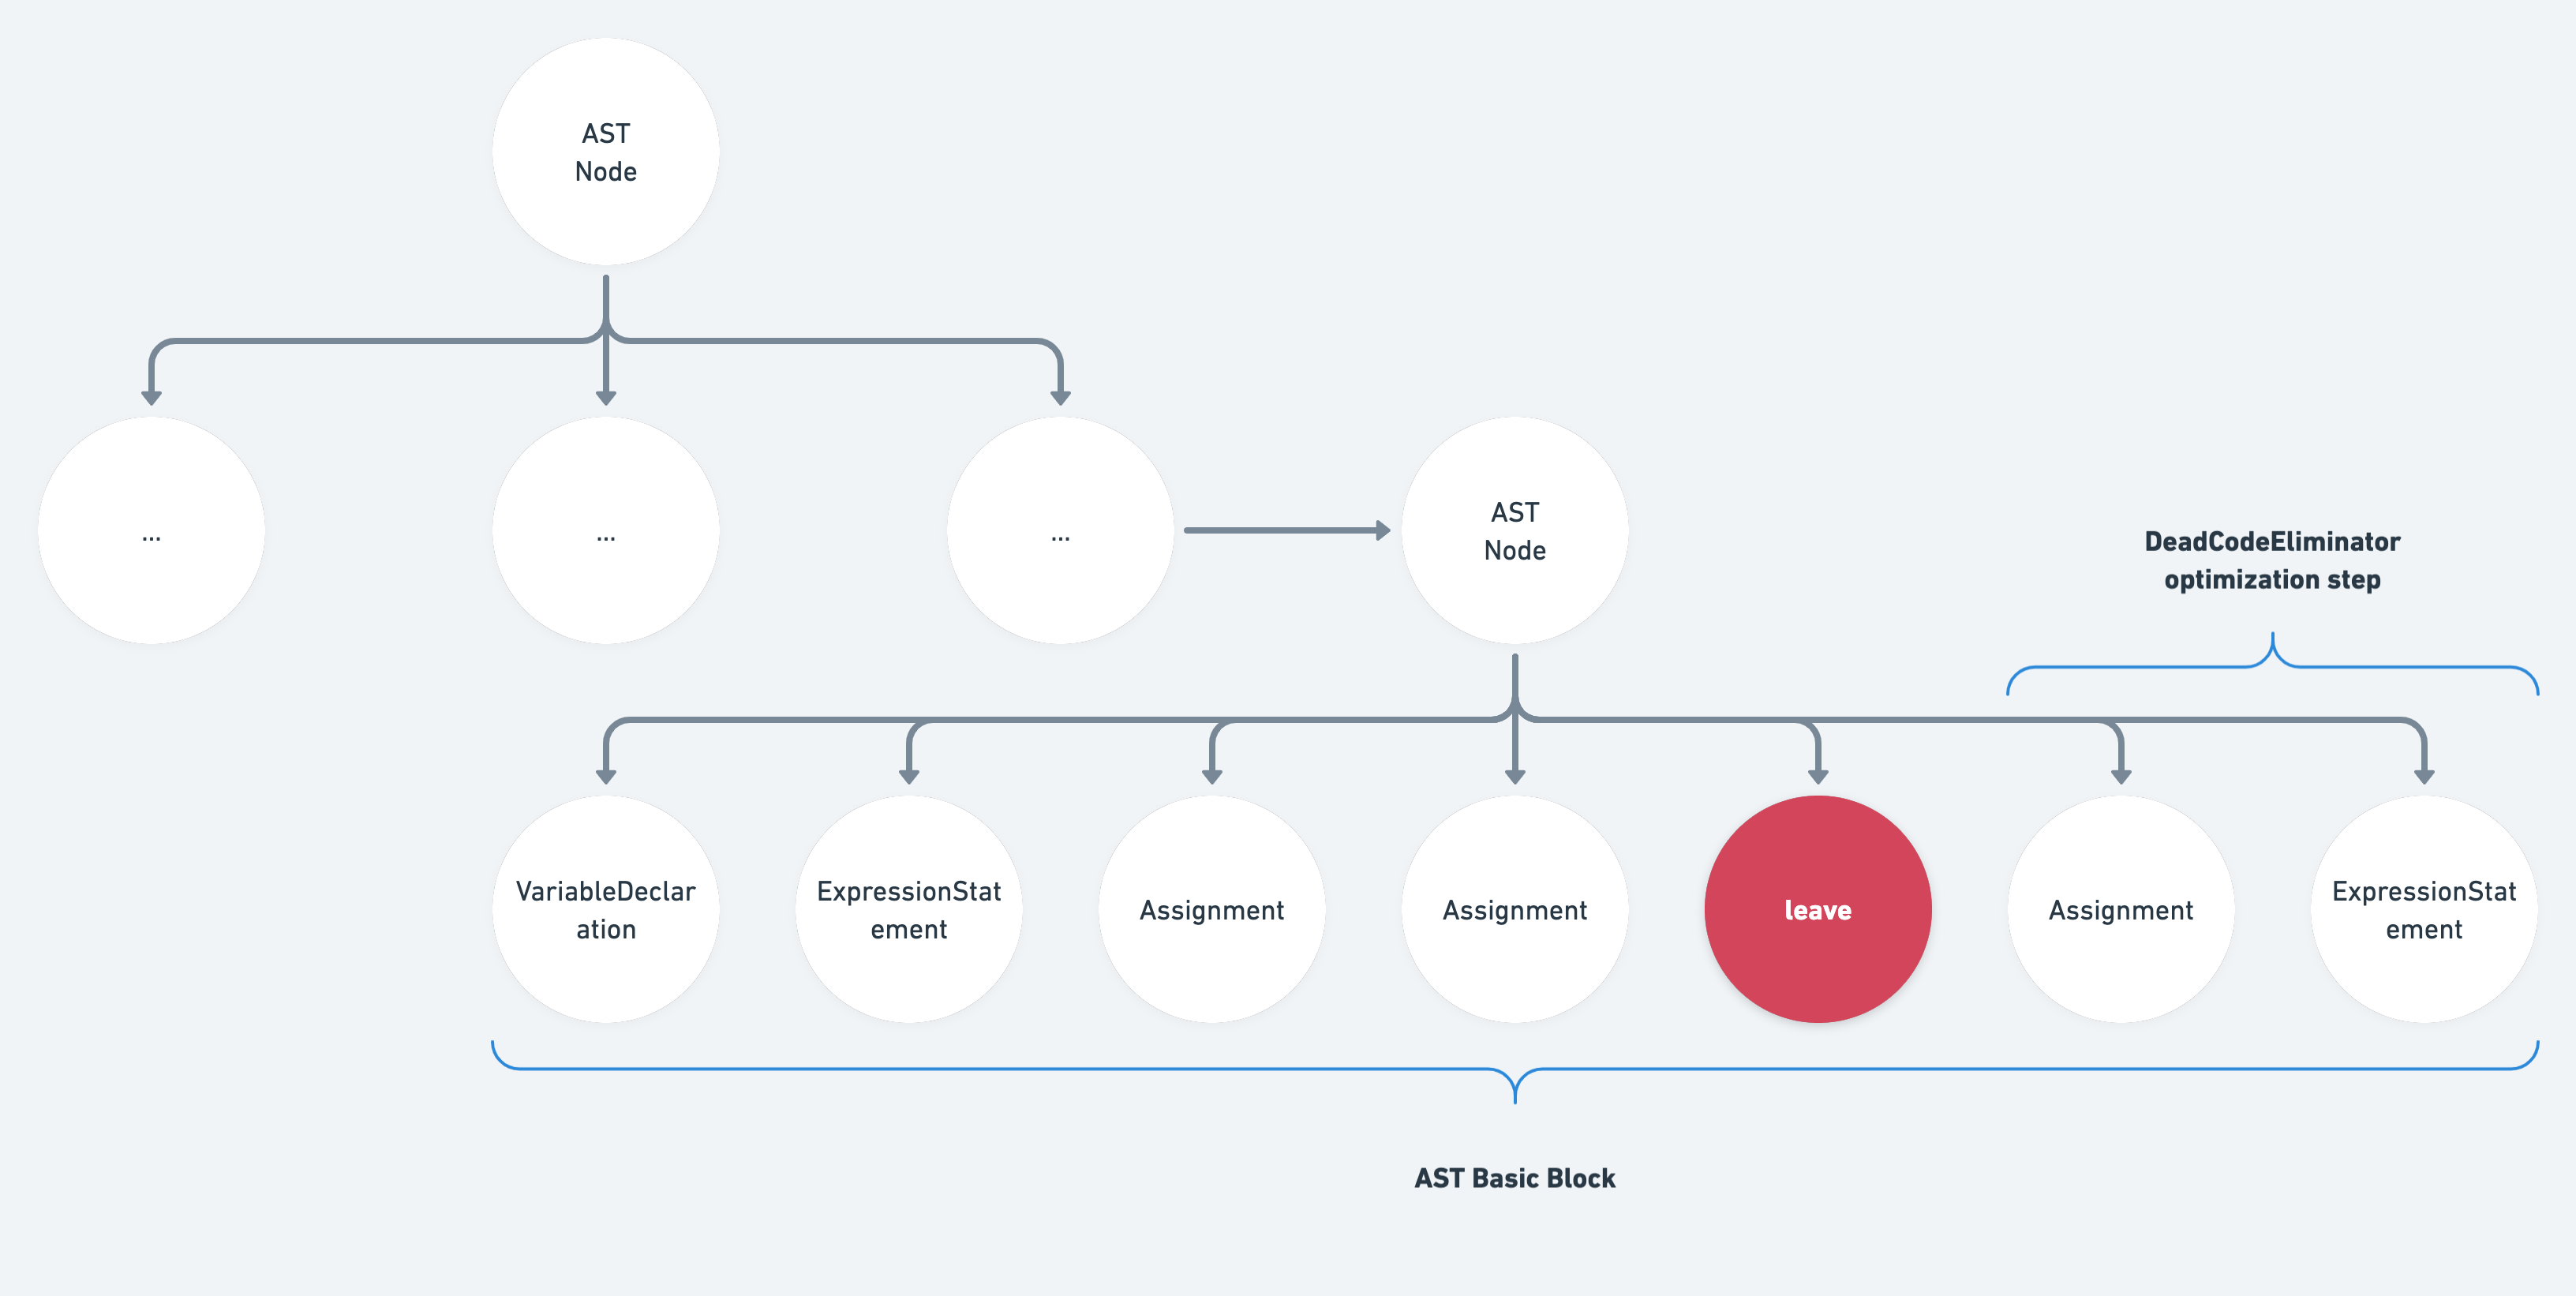
\includegraphics[width=\textwidth]{images/basic_block_termination_ast_example.png}
    \caption{Example of termination flow inside a YUL AST's basic block node. DeadCodeEliminator is used to prune unreachable code}
    \label{fig:basic-block-termination-ast-example}
\end{figure}

\paragraph*{}
With this simplification in mind, the edge case can be handled by enhancing the \\ \lstinline[columns=fixed]{UnusedAssignEliminator.visit} function for Basic Blocks in the YUL AST. That is, when visiting the block, we make a copy of the current recorded assignments (outside of the current basic block) such that after visiting we can compute the new assignments - this includes variable declarations. If basic block $B$'s body trailing statement induces a termination flow, then we can safely remove all of the new assignments made in that block, even if they are referenced in another block of the CFG.

\paragraph*{}
Some special cases must be considered however, such as \textbf{state variables} which are persistent within the contract. These are defined in Solidity as members of the smart contract. Obviously, any assignment to such a persistent variable $p$ \textbf{should not} be removed, regardless of the control flows that follows it. The only case in which we can safely remove them is if they consist unreachable code, which the DeadCodeEliminator will handle. We therefore restrict the behaviour of the above enhancement to only local basic block variables or to the inputs of the basic block \footnote{This is actually easy to do because persistent variables are kept in memory. Their values are updated via function calls, which are not recognized by the AST walker as variable assignments / declarations.}.

\paragraph*{}
The Solidity compiler reports that the estimated gas usage for the contract construction for code sample \ref*{code:unused-assign-eliminator-handle-termination-flow} went down from $67723$ to $65723$, a saving of $2000$ gas. Also, the execution of the \lstinline[columns=fixed]{assignBeforeTermination} function went down from $2585$ to $2565$, which is $20$ gas less. The result of the enhancement can be seen in figure \ref{fig:unused-assign-eliminator-handle-termination-flow} where the full optimizer suite was ran against the same code sample, with and without the above enhancement. This also enabled StructuralSimplifier to simplify code further, completely removing the second \lstinline[columns=fixed]{if} condition and un-nesting the emitting of the \lstinline[columns=fixed]{BalanceIsEmpty} event.


\begin{figure}
    \centering
    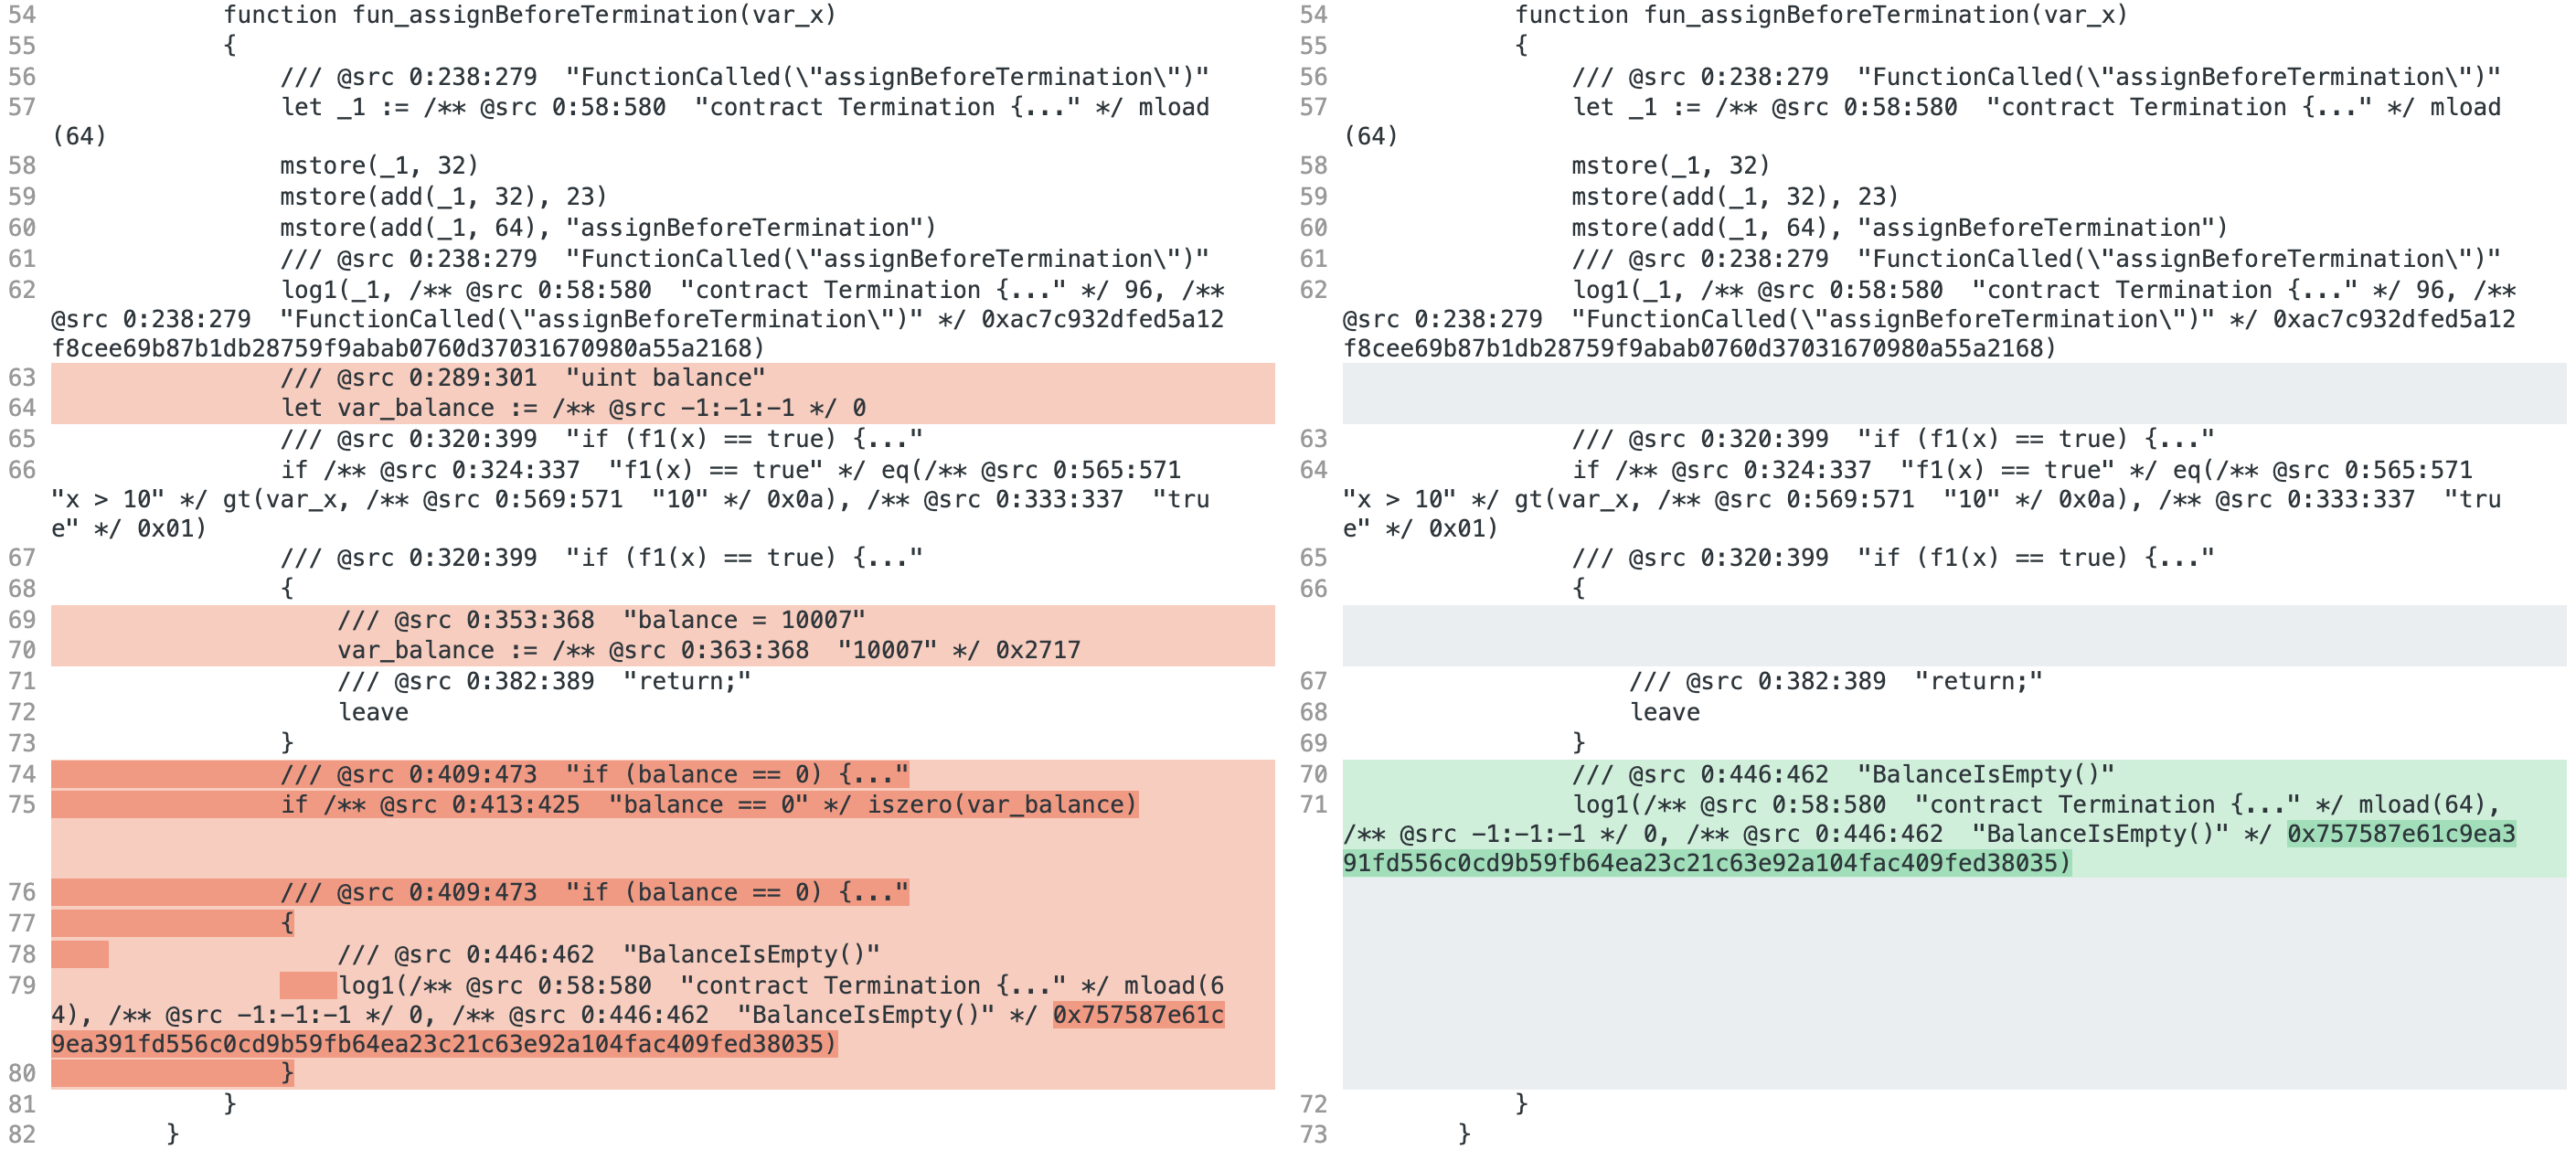
\includegraphics[width=\textwidth]{images/unused_assign_eliminator_handle_termination_flow.png}
    \caption{Full optimizer suite ran against code sample \ref{code:unused-assign-eliminator-handle-termination-flow}. The right hand side YUL IR handles termination flows within basic blocks for variable assignments and declarations.}
    \label{fig:unused-assign-eliminator-handle-termination-flow}
\end{figure}


\section{Pruning redundant termination flows}
\paragraph*{}
As stated in the previous chapter, running an optimization step $X$ may give more opportunities to optimization step $Y$ to further enhance the YUL IR (therefore the resulted bytecode). This was the case for the above enhancement, where experiments pointed out that if a basic block contains a trailing \lstinline[columns=fixed]{if} statement, then pruning code inside the \lstinline[columns=fixed]{if}'s body may result in a single trailing, redundant \lstinline[columns=fixed]{leave} instruction within the body. The expected basic block pattern for this case is
\begin{lstlisting}
    { ... if (C) { leave } }
\end{lstlisting}
after the removal of redundant code has been done.

\label{structural-simplifier-cascading-example}
\paragraph*{}
A good solution for this edge case was changing how the StructuralSimplifier works and make it look for \lstinline[columns=fixed]{leave} statements within an \lstinline[columns=fixed]{if}'s body. If that's the case, then the \lstinline[columns=fixed]{leave} statement is simply removed. This enabled for cascading enhancements, and the StructuralSimplifier will further completely remove the \lstinline[columns=fixed]{if} condition and body and replace it with the operations inside the condition itself. The removal of the \lstinline[columns=fixed]{leave} statement did not improve gas usage significantly, but the cascading optimization aspect is what enables true optimization opportunities here.

% \section{Handling termination flows in DataFlowAnalyzer}
% \paragraph*{}
% A way to ``scale up'' the enhancements done
% Un tool folosit de alti optimizer. Important sa reflecte starea corecta a programului. De ce? Ca sa poata faca computare corecta la compile time.

% \section{Pruning redundant function calls}
% \paragraph*{}
% Mai grelut.